In this chapter we introduce a novel readout technology at the pixel level for LArTPCs. 
The basic readout circuit was first introduced by \citep{qpix:nygren:mei}.

Pixel based readouts offer several advantages over the traditional wire readout \citep{lartpc_recon_problems_joshi_2015}.
The key improvement offered is true 3-D image reconstruction. 
This allows for sharper vertex reconstruction, thereby improving the overall resolution of DUNE and decreasing the required time for a NP measurement.
Other advantages rely on data analysis and data storage. 
A pixel based readout automatically records 2 of the three spatial dimensions, and thereby provides for simpler analysis.
Additionally, the pixelated readout method presented here cuts the total required data storage and data acquisition rate (without loss to precision) by several orders of magnitude.

However, the advantages also come with the cost of increased design complexity as the number of readout channels increases by more than three orders of magnitude. 
The traditional wire based readout within a DUNE module will include hundreds to thousands of channels, whereas a full DUNE module with a pixel-based readout will have 10's of millions of channels.
This number of required channels to be stably readout during DUNE's expected lifetime ($> 10$ years), where the electronics continually operate at liquid argon temperatures is likely the largest hurtle for a pixel-based design.
The aim of this dissertation is to address the channel-size problem.

\section{Q-Pix: The Circuit Level Design}

Concept of this combined ASIC and reducing the number of channels relies on digital multiplexing.

This differs from other concepts such as Genetic Multiplexing (\citep{PROCUREUR2013888_genetic_multiplexing}) and using only regions of interest (ROI).

\begin{figure}[ht!]
\centering
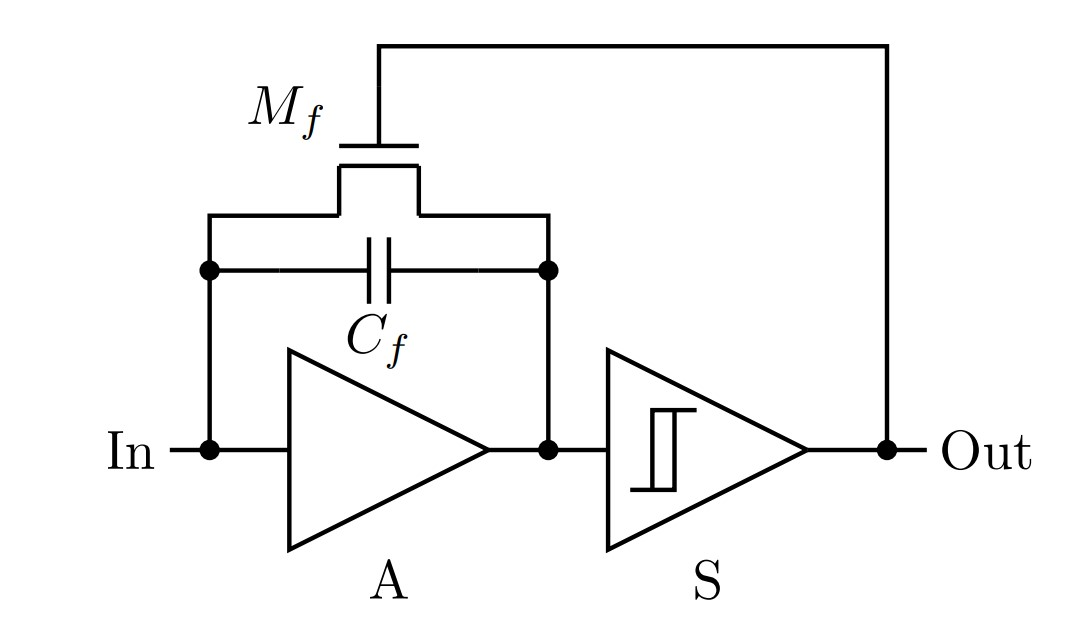
\includegraphics[width=\textwidth]{images/qpix_circuit.jpg}
\caption{Image of Basic Q-Pix Readout circuit. Currently this is being designed within a custom analog ASIC. Image is taken from \citep{qpix:nygren:mei}.}
\end{figure}


\begin{figure}[ht!]
\centering
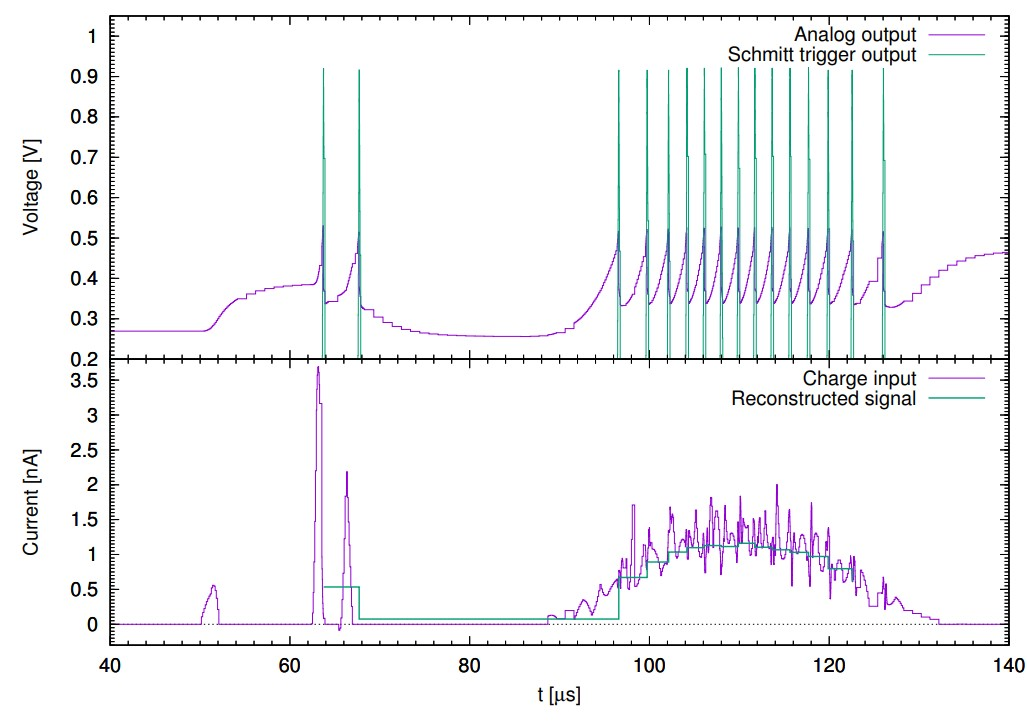
\includegraphics[width=\textwidth]{images/qpix_rtd_reconstruction_example.jpg}
\caption{Example reconstruction of the reset time difference (RTD) based on the Q-Pix readout design. Image is taken from \citep{qpix:nygren:mei}.}
\end{figure}

\begin{figure}[ht!]
\centering
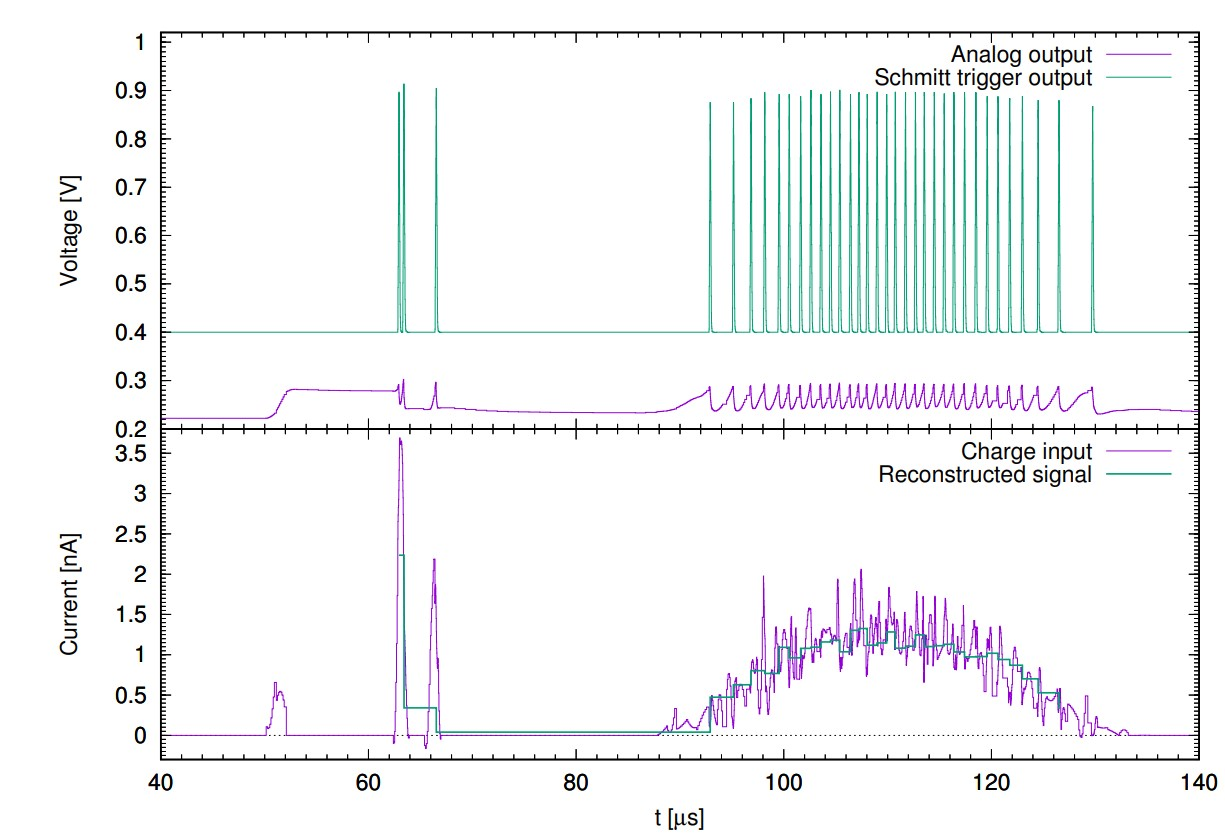
\includegraphics[width=\textwidth]{images/qpix_rtd_reconstruction_example_03fc.jpg}
\caption{Example reconstruction of the reset time difference (RTD) based on the Q-Pix readout design. delta-Q was chosen to be $0.3 fC$. Image is taken from \citep{qpix:nygren:mei}.}
\end{figure}

\section{System Requirements}

\section{How Q-Pix fits into a DUNE APA}

DUNE Anode Plane Assemblies (APA) designs are based on \citep{DUNE-FD_TDRv4:Abi_2020}.

%% example image of DUNE-APA from DUNE-FD TDR.
\begin{figure}[ht!]
\centering
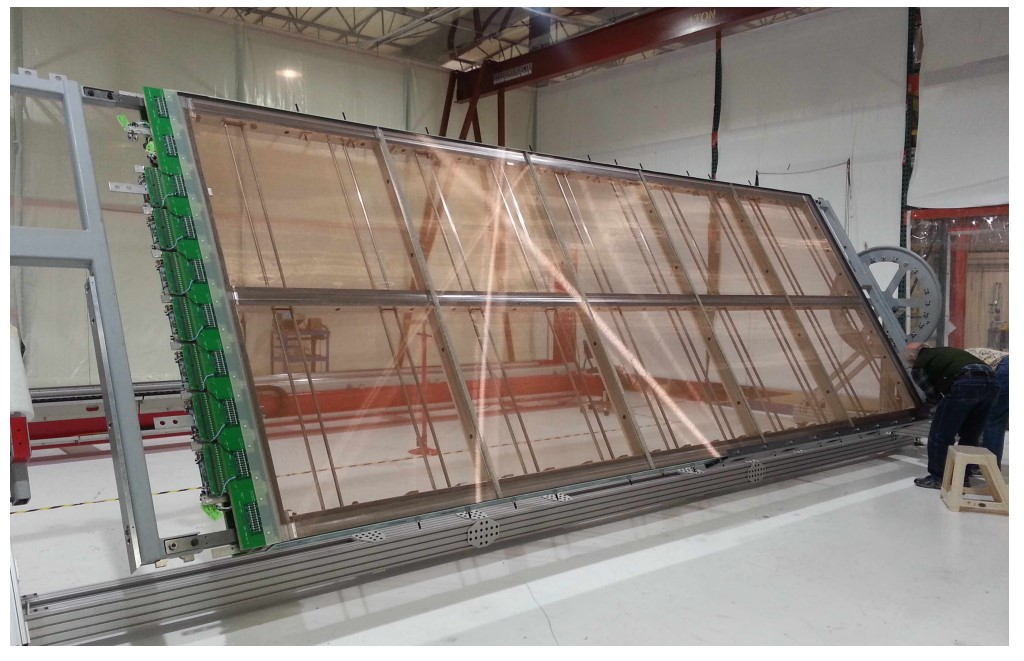
\includegraphics[width=\textwidth]{images/dune_fd_tdr_apa_image.jpg}
\caption{A simple caption \citep{DUNE-FD_TDRv4:Abi_2020}}
\end{figure}
